%Since all tasks share the same underlying model $\beta$, we use a simplified objective as follows.
%\begin{align}
%	\label{eq_mtl_basic}
%	f(w) = \sum_{i=1}^k \norm{X_i w - Y_i}^2.
%\end{align}
%{\bf The distributed learning problem.}
%    \begin{align}
%     f(w) = \sum_{i=1}^k \normFro{X_i w - Y_i}^2. \label{eq_dist}
%   \end{align}
%Equation \eqref{eq_mtl_basic} is simplified from equation \eqref{eq_mtl} by setting $A_i$ to be 1 for all tasks. %can select a model from the subspace of $B$ to fit $(X_i, Y_i)$.

As a warm up, we show that when $\beta_s = \beta_t$, then the transfer is always positive.

\begin{proposition}\label{prop_monotone}
	Suppose that $n > p$.
  When there is no model shift, i.e. $\beta_s = \beta_t$, adding the source task data always reduces the estimation error and the test error for the target task, i.e.
	\begin{align}
%		\err(\hat{\beta}_{t}^{\MTL})  &\le \err(\hat{\beta}_t^{\STL}), \text{ and} \label{eq_mono_e}\\
		\te(\hat{\beta}_{t}^{\MTL}) &\le \te(\hat{\beta}_t^{\STL}). \label{eq_mono_te}
	\end{align}
\end{proposition}

\begin{proof}
%	Equation \eqref{eq_mono_e} is simply because
%		\[ \err(\hat{\beta}_{s,t}) = \bigtr{(X_1^{\top}X_1 + X_2^{\top}X_2)^{-1}} \le \bigtr{(X_1^{\top}X_1)^{-1}} = \err(\hat{\beta}_t). \]
%	Equation \eqref{eq_mono_te} follows because
	Recall that $\hat{\beta}_t^{\MTL} = \hat{w} \cdot \hat{B}$.
	By the optimality of $\hat{w}$, we have by setting $w = 1$ in equation \eqref{eq_te_mtl}
	\begin{align*}
		\te(\hat{\beta}_t^{\MTL}) &\le \sigma^2 \cdot \bigtr{(X_1^{\top}X_1 + X_2^{\top}X_2)^{-1}\Sigma_2} \\
		&= \sigma^2 \cdot \bigtr{\bigbrace{\Sigma_2^{-1/2}X_1^{\top}X_1\Sigma_2^{-1/2} + \Sigma_2^{-1/2}X_2^{\top}X_2\Sigma^{-1/2}}^{-1}} \\
		&\le \bigtr{\bigbrace{\Sigma_2^{-1/2}X_2^{\top}X_2\Sigma_2^{-1/2}}^{-1}}
			= \bigtr{(X_2^{\top}X_2)^{-1} \Sigma_2} = \te(\hat{\beta}_t^{\STL}),
	\end{align*}
	which concludes the proof.
\end{proof}

As a remark, we can derive a similar result for the estimation error as well. The details are omitted.


In the above, the first is a bias term introduced by the model shift between the source and target tasks.
The second is a variance term, which decreases monotonically as we add more and more source task data.
Let $\hat{w}$ denote the minimizer of $te(w_2 \hat{B})$ over $w\in\real$.
Note that we can obtain the value of $\te(w_1\hat{B})$ through a validation set.
We will denote $\hat{\beta}_t^{\TL} = w_2 \hat{B}(\hat{w})$.

There are two reasons for studying this setting.
First, this is akin to performing transfer learning using the hard parameter sharing architecture.
Another way to obtain $\hat{\beta}_t^{\TL}$ is that once we minimize the multi-task validation loss, we further minimize the validation loss on the target dataset, which is also known as fine-tuning in practice.
%	\begin{align}
%		\left(\frac{n_2}{n_1+n_2}\frac1{a_1^2}- \frac1{n_1+n_2}\sum_{i=1}^p \frac{1}{ (a_1 + \lambda_i^2a_2)^2  }\right) a_3 -  \left(\frac1{n_1+n_2}\sum_{i=1}^p \frac{  \lambda_i^2 }{ (  a_1 + \lambda_i^2a_2)^2  }\right)a_4 &=  \frac1{n_1+n_2}\sum_{i=1}^p \frac{1 }{ (  a_1 + \lambda_i^2a_2)^2  } , \label{eq_a3} \\
%		\left( \frac{n_1}{n_1+n_2}\frac1{a_2^2} -  \frac1n\sum_{i=1}^p \frac{\lambda_i^4   }{  (a_1 + \lambda_i^2a_2)^2  }\right)a_4 -\left( \frac1 {n_1+n_2}\sum_{i=1}^p \frac{\lambda_i^2  }{  (a_1 + \lambda_i^2a_2)^2  }\right)a_3 &=   \frac1 {n_1+n_2}\sum_{i=1}^p \frac{\lambda_i^2 }{  (a_1 + \lambda_i^2a_2)^2  }. \label{eq_a4}
%	\end{align}
	%We have that
	%\begin{align*}
	%	&~ {\bignorm{\Sigma_2^{1/2} (X_1^{\top}X_1 + X_2^{\top}X_2)^{-1} X_1^{\top}X_1 %(\beta_s - \beta_t)}} \\
	%	&\le ~ \left[(\beta_s - \beta_t)^{\top}\Sigma_1^{1/2}M\frac{(1 + a_3)\id + a_4 M^{\top}M}{(a_1 + a_2 M^{\top}M)} M^{\top}\Sigma_1^{1/2} (\beta_s - \beta_t)\right]^{1/2} \\
	%	&+ \left\|M\frac{(1 + a_3)\id + a_4 M^{\top}M}{(a_1 + a_2 M^{\top}M)} M^{\top}\right\|_{op}^{1/2} \|\Sigma_1^{1/2} (\beta_s - \beta_t)\|_2 \left( 2\sqrt{\frac{p} {n_1}} + \frac{p}{n_1}\right),
	%\end{align*}
	%and
	%\begin{align*}
	%	&~ {\bignorm{\Sigma_2^{1/2} (X_1^{\top}X_1 + X_2^{\top}X_2)^{-1} X_1^{\top}X_1 (\beta_s - \beta_t)}} \\
	%	&\ge ~ \left[(\beta_s - \beta_t)^{\top}\Sigma_1^{1/2}M\frac{(1 + a_3)\id + a_4 M^{\top}M}{(a_1 + a_2 M^{\top}M)} M^{\top}\Sigma_1^{1/2} (\beta_s - \beta_t)\right]^{1/2} \\
	%	&- \left\|M\frac{(1 + a_3)\id + a_4 M^{\top}M}{(a_1 + a_2 M^{\top}M)} M^{\top}\right\|_{op}^{1/2} \|\Sigma_1^{1/2} (\beta_s - \beta_t)\|_2 \left( 2\sqrt{\frac{p} {n_1}} + \frac{p}{n_1}\right).
	%\end{align*}
	%Here in the error term $p$ can be replaced with the rank of $\Sigma_1$. Without any extra information, we can only use the fact the rank of $\Sigma_1$ is at most $p$.



%Then it is equivalent to study
%$$Q:=  ( X_1^T X_1 )^{-1}   D X_2^T X_2 D ,$$
%which has the same nonzero eigenvalues of
%$$\mathcal Q:=  X_2 D ( X_1^T X_1 )^{-1} D X_2^T,$$
%i.e. $\mathcal Q$ has the same nonzero eigenvalues of $Q$, but has $(n_2-p)$ more zero eigenvalues.

%----------The following is the results on the eigenvalues, not the singular values-------------
%We are interested in the eigenvalues of
%$$(X_1^{\top}X_1)^{-1} (X_2^{\top}X_2),$$
%which is called a generalized Fisher matrix. As in the previous setting, we write out their covariance explicitly and consider
%$$  (\Sigma_1^{1/2}  Z_1^T Z_1 \Sigma_1^{1/2})^{-1}   \Sigma_2^{1/2}  Z_2^T Z_2 \Sigma_2^{1/2} ,$$
%where $\Sigma_{1,2}$ are $p\times p$ deterministic covariance matrices, and $X_1=(x_{ij})_{1\le i \le n_1, 1\le j \le p}$ and $X_2=(x_{ij})_{n_1+1\le i \le n_1+n_2, 1\le j \le p}$ are $n_1\times p$ and $n_2 \times p$ random matrices, respectively, where the entries $x_{ij}$, $1 \leq i \leq n_1+n_2\equiv n$, $1 \leq j \leq p$, are real independent random variables satisfying \eqref{eq_12moment}.
%We can study it using the linearization matrix ({\color{red}for my own purpose right now})
%$$ H = \begin{pmatrix} - z I & X_2D & 0 \\ DX_2^T & 0 & X_1^T \\ 0 & X_1 & I \end{pmatrix}, \quad G(z):=H(z)^{-1}.$$
%Then the $(1,1)$-th block is equal to $\cal G(z):=(\mathcal Q-z)^{-1}$. We denote
%\begin{equation}\label{m1m}m_1(z):=\frac1n\tr \cal G(z), \quad m(z)= \frac1p \left[ nm_1(z) + \frac{n_2-p}{z}\right].\ee
%We can show that it satisfies the following self-consistent equations together with another $m_3(z)$:
%\begin{align}\label{m13}
%\frac{n_2}{n}\frac1{m_1} = - z +\frac1n\sum_{i=1}^p \frac{d_i^2}{ m_3 + d_i^2m_1  } ,\quad \frac{n_1}{n}\frac1{m_3} = 1 +\frac1n\sum_{i=1}^p \frac{1}{   m_3 + d_i^2m_1  } .
%\end{align}
%For these two equations, we can obtain one single equation for $m_1(z)$:
%\begin{align}\label{m1}
%m_3= 1-\frac pn + zm_1, \quad \frac{n_2}{n}\frac1{m_1} = - z +\frac1n\sum_{i=1}^p \frac{d_i^2}{ 1-\frac pn + (z + d_i^2)m_1  }  .
%\end{align}
%One can solve the above equation for $m_1$ with positive imaginary parts, and then calculate $m(z)$ using \eqref{m1m}.
%
%With $m(z)$, we can define
%$$\rho_c(z):=\frac1\pi \lim_{\eta\downarrow 0} m(z).$$
%It will be a compact supported probability density which gives the eigenvalue distribution of $Q$. Moreover, we have
%$$\frac{1}{p}\tr \frac1{(\Sigma_1^{1/2}  X_1^T X_1 \Sigma_1^{1/2})^{-1}   \Sigma_2^{1/2}  X_2^T X_2 \Sigma_2^{1/2} +1}\left(\frac1{(\Sigma_1^{1/2}  X_1^T X_1 \Sigma_1^{1/2})^{-1}   \Sigma_2^{1/2}  X_2^T X_2 \Sigma_2^{1/2} +1}\right)^T \approx \int \frac{\rho_c(x)}{(x+1)^2}{\rm d}x.$$
%We know that
%$$ m(z)=\int \frac{\rho_c(x)}{ x-z}{\rm d}x.$$
%Hence we have
%$$ m'(-1)=\int \frac{\rho_c(x)}{(x+1)^2}{\rm d}x.$$
%
%Moreover, the right edge $\lambda_+$ of $\rho_c$ gives the location of the largest eigenvalue, while the left edge $\lambda_-$  of $\rho_c$ gives the location of the smallest eigenvalue. They will provide the upper and lower bounds on the operator norm:
%$$\frac{1}{1+\lambda_+}\le \frac1{(\Sigma_1^{1/2}  X_1^T X_1 \Sigma_1^{1/2})^{-1}   \Sigma_2^{1/2}  X_2^T X_2 \Sigma_2^{1/2} +1}\le \frac1{1+\lambda_-}.$$
%The edges of the spectrum can be determined by solving the following equations of $(x,m_1)$:
%$$\frac{n_2}{n}\frac1{m_1} = - x +\frac1n\sum_{i=1}^p \frac{d_i^2}{ 1-\frac pn + (x + d_i^2)m_1  } ,\quad  \frac{n_2}{n}\frac1{m_1^2} = \frac1n\sum_{i=1}^p \frac{d_i^2 (x+d_i^2)}{\left[ 1-\frac pn + (x + d_i^2)m_1 \right]^2 } .$$
%The solutions for $x$ give the locations for the edges of the spectrum.
%--------------------------------------





%\section{The Case of Two Tasks}\label{sec_defspike}
%We denote task 1 as the source, i.e. $\beta_1 = \beta_s$.
%\subsection{Covariate Shift}
%\subsection{Model Shift}
	Moreover, when $n_1 = 0$, we have %we have that $a_1 = 0$ and $a_2 = (n_2-p) / n_2$, hence
	\begin{align}\label{lem_cov_shift_eq2} \bigtr{(X_2^{\top}X_2)^{-1}\Sigma_2} = \frac{p}{n_2-p} + \bigo{n^{-1/2+\epsilon}}, \end{align}
which is a well-known result for inverse Whishart matrices {\color{red}add some references}.
 %, where $a_{3,4}$ are found using equations in  \eqref{m35reduced}.


%Hence the task models have distance $d^2\cdot p$ in expectation.
%	We first consider $\Sigma_2 = \id$. In this case, we can simplify $\Delta_{\beta}$ as follows
%	\begin{align} \label{eq_delta_simple}
%		\Delta_{\beta} \define d^2 \cdot \sum_{i=1}^p \frac{(1 + a_3)\lambda_i^2 + a_4
%\lambda_i^4}{(a_1 \lambda_i^2 + a_2)^2}.
%	\end{align}

%{\color{blue}if $\Sigma_1=\Sigma_2=\id$, then
%	\begin{align}
%		a_1 = c_1 \left( 1- \gamma_n\right) , \quad
%		a_2 = c_2 \left( 1- \gamma_n\right), \quad
%		a_3 = \frac{\gamma_n c_2}{1-\gamma_n}, \quad
%		a_4 =  \frac{\gamma_n c_1}{1-\gamma_n}.
%	\end{align}
%	where $\gamma_n=p/n$, $c_1=n_1/n$, and $c_2=n_2/n$.
%}

	%Then we obtain
	%\begin{align}
	%	\Delta_{\beta} = p \cdot d^2 \cdot \frac{c_1^2 (c_1 + c_2)}{(c_1 + c_2 - 1)^3},
	%	\Delta_{\vari} = \sigma^2 \cdot \frac{c_1}{(c_2 - 1)(c_1 + c_2 - 1)}.
	%\end{align}


<<<<<<< HEAD
%\paragraph{A tighter bound for a special case.}
Under the setting of Proposition \ref{prop_dist_transition}, we can get a bound tighter than Theorem \ref{thm_model_shift} as follows.

	\begin{proposition}\label{prop_model_shift_tight}
		In the setting of Theorem \ref{thm_model_shift}, assume that $\Sigma_1 =\id$,
		$\beta_t$ is i.i.d. with mean $0$ and variance $\kappa^2$ and $\beta_s - \beta_t$ is i.i.d. with mean $0$ and variance $d^2$.
		We set $\Delta_{\beta} = \bigbrace{(1 - \hat{w})^2 \kappa^2 + d^2)} \bigtr{Z}$
		and we have
		\begin{align*}
			\te(\hat{\beta}_t^{\MTL}) \le \te(\hat{\beta}_t^{\STL}) \text{ when: } & \Delta_{\vari} \ge \bigbrace{1 + \sqrt{\frac{p}{n_1}}}^4 \Delta_{\beta}, \\
			\te(\hat{\beta}_t^{\MTL}) \ge \te(\hat{\beta}_t^{\STL}) \text{ when: } & \Delta_{\vari} \le \bigbrace{1 - \sqrt{\frac{p}{n_1}}}^4 \Delta_{\beta}.
		\end{align*}
	\end{proposition}
We will give the proof of this proposition after proving Theorem \ref{thm_model_shift} in Section \ref{sec pfmain}	.

Using Lemma \ref{lem_minv} and \ref{lem_cov_shift}, we can track the change of variance from $\hat{\beta}_t^{\MTL}$ to $\hat{\beta}_t^{\STL}$ as follows.

\begin{lemma}\label{lem_hat_v}
	Recall that $\hat{v} = \hat{w_1} / \hat{w_2}$.
	In the setting of Proposition \ref{prop_dist_transition}, we have that
	\[ \abs{\hat{v} - 1} \lesssim \frac 1 p. \]
\end{lemma}

<<<<<<< HEAD
=======
Hence the task models have distance $d^2\cdot p$ in expectation.
	We first consider $\Sigma_2 = \id$. In this case, we can simplify $\Delta_{\beta}$ as follows
	\begin{align} \label{eq_delta_simple}
		\Delta_{\beta} \define d^2 \cdot \sum_{i=1}^p \frac{(1 + a_3)\lambda_i^2 + a_4 \lambda_i^4}{(a_1 \lambda_i^2 + a_2)^2}.
	\end{align}
	Now we solve the equations \eqref{eq_a2}, \eqref{eq_a3}, \eqref{eq_a4} to get
	\begin{align}
		a_1 = \frac{c_1(c_1 + c_2 - 1)}{(c_1 + c_2)^2},
		a_2 = \frac{c_2(c_1 + c_2 - 1)}{(c_1 + c_2)^2},
		a_3 = \frac{c_2}{(c_1 + c_2)(c_1 + c_2 - 1)},
		a_4 = \frac{c_1}{(c_1 + c_2)(c_1 + c_2 - 1)}.
	\end{align}
%{\color{blue}if $\Sigma_1=\Sigma_2=\id$, then
%	\begin{align}
%		a_1 = c_1 \left( 1- \gamma_n\right) , \quad
%		a_2 = c_2 \left( 1- \gamma_n\right), \quad
%		a_3 = \frac{\gamma_n c_2}{1-\gamma_n}, \quad
%		a_4 =  \frac{\gamma_n c_1}{1-\gamma_n}.
%	\end{align}
%	where $\gamma_n=p/n$, $c_1=n_1/n$, and $c_2=n_2/n$.
%}

	Then we obtain
	\begin{align}
		\Delta_{\beta} = p \cdot d^2 \cdot \frac{c_1^2 (c_1 + c_2)}{(c_1 + c_2 - 1)^3},
		\Delta_{\vari} = \sigma^2 \cdot \frac{c_1}{(c_2 - 1)(c_1 + c_2 - 1)}.
	\end{align}


%\begin{example}[\textbf{When $\Sigma_1 = \Sigma_2$}]
%In this case, we have $\lambda_i = 1$ for all $1\le i\le p$.
%And $a_1 + a_2 = 1 - p / (n_1 + n_2)$.
%Hence
%\[ \te(\hat{\beta}_{s,t}) = \frac{\sigma^2 p^2}{n_1 + n_2 - p} \text{ and } \err(\hat{\beta}_{s,t}) = \frac {\sigma^2 p} {n_1 + n_2 - p} \bigtr{\Sigma_2^{-1}}. \]
%\end{example}

\paragraph{Extending the intuition to the general case.}
When there is model shift, i.e. $\beta_s = \beta_t$, we can still use Theorem \ref{thm_model_shift} (and Proposition \ref{prop_model_shift_tight}) to get the result.
\begin{itemize}
	\item \textbf{The effect of covariate shift:}
	\item \textbf{The effect of data ratio:}
\end{itemize}


%	\centering
%	\begin{minipage}{0.48\textwidth}
%		\centering
%		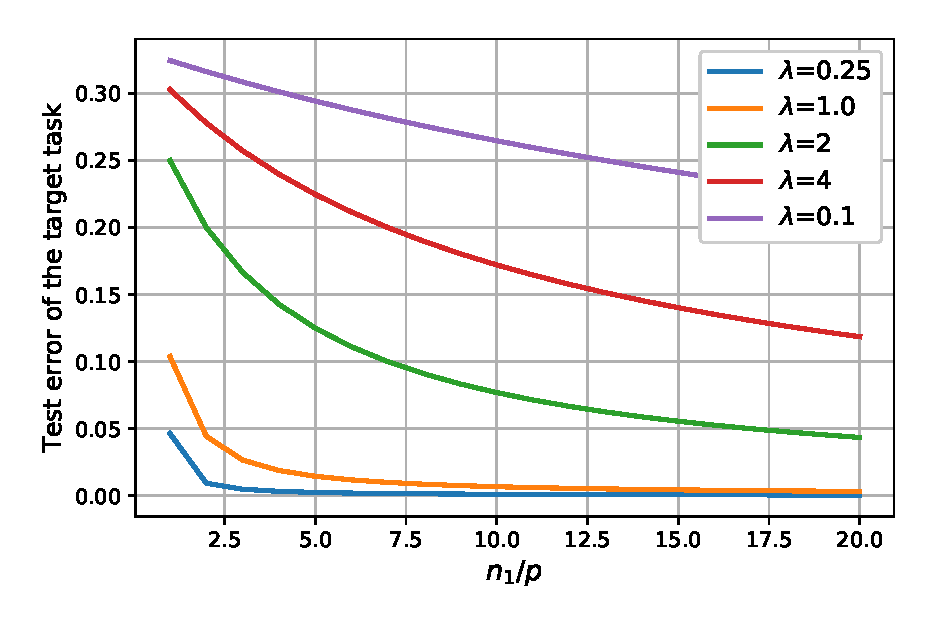
\includegraphics[width=0.9\textwidth]{figures/scaling.eps}
%		\caption{When $\Sigma_1 = \Sigma_2 / \lambda$.}
%		\label{fig_te_scaling}
%	\end{minipage}\hfill

	%, because otherwise $aM$ always achieves a smaller error than $M$ for $a>1$. For this purpose, we introduce the following condition

	%	for some constant $a>0$, and compare different choices of $M$ under this constraint. The next proposition shows that, roughly speaking, as long as there are sufficiently many source task datas, then $M=a\id$ always gives (approximately) the smallest test error.
%\smallskip
%\begin{example}[\textbf{When $\Sigma_1 = \Sigma_2 / \lambda$}]
%In this case, equations \eqref{eq_a2} become
%\[ a_1 + a_2 = 1 - p/(n_1 + n_2), a_1 + \frac{p}{n_1 + n_2} \cdot \frac {a_1} {a_1 + \lambda^2 a_2} = \frac{n_1} {n_1 + n_2}. \]
%By solving these, we can get the test errors (the estimation error behaves
%similarly).
%Figure \ref{fig_te_scaling} shows how they grow as we increase the number of source task data points.
%Here $n_2 = 4p$ and $n_1$ ranges from $p$ to $20p$.
%We can see that the smaller $\lambda$ is, the lower the test errors will be.
%\end{example}

%	{\color{blue}To write the bounds in the form \eqref{upper} and \eqref{lower}, we have to define $\wh w$ as the minimizer of
%	$$\frac{\sigma^2}{n_1 + n_2} \bigtr{\frac1{a_1(w) M(w)^{\top}M(w) + a_2(w)\id}}+ \Delta_\beta(w).$$
%	Otherwise, the two bounds has to be written into the form
%	\begin{align*}
%	{\sigma^2}\frac{p}{n_2 - p}\ge \min_w \left\{\frac{\sigma^2}{n_1 + n_2} \bigtr{\frac1{a_1(w) M(w)^{\top}M(w) + a_2(w)\id}} + \Delta_\beta(w)+ \left(\bigbrace{1 + \sqrt{\frac{p} {n_1}}}^4 - 1 \right) \delta(w)\right\},
%	\end{align*}
%	and
%	\begin{align*}
%	{\sigma^2}\frac{p}{n_2 - p}\le \min_w \left\{\frac{\sigma^2}{n_1 + n_2} \bigtr{\frac1{a_1(w) M(w)^{\top}M(w) + a_2(w)\id}}+ \Delta_\beta(w) - 2\bigbrace{2\sqrt{\frac {p}{n_1}} + \frac{p}{n_1}} \delta(w)\right\}.
%	\end{align*}
%	}

%\begin{figure}
%	\begin{minipage}{0.48\textwidth}
%		\centering
%		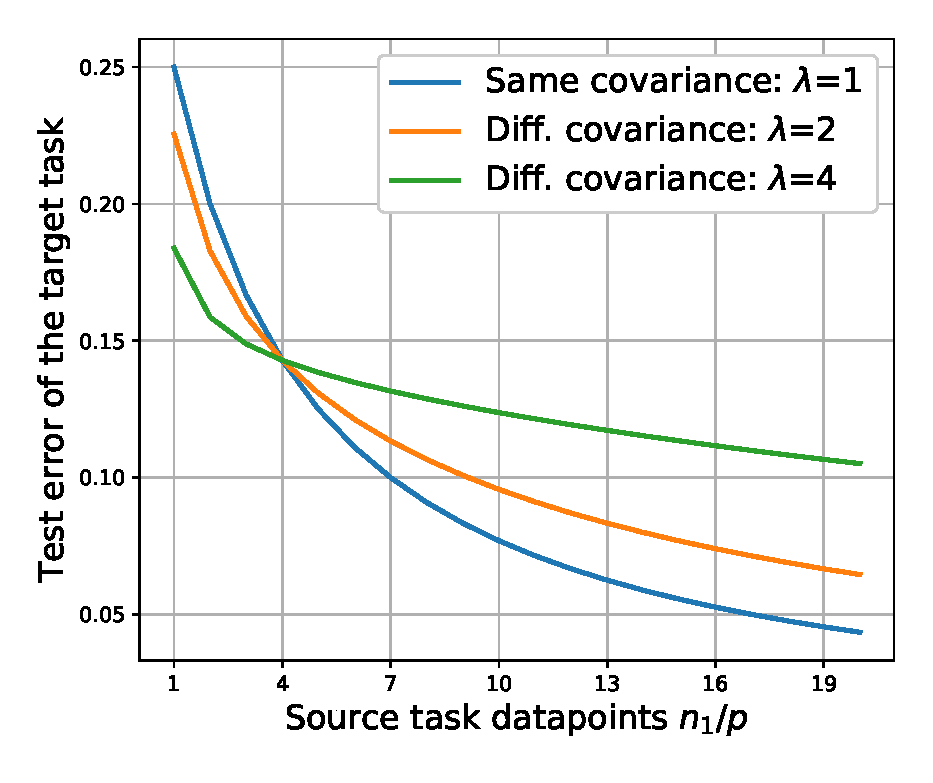
\includegraphics[width=0.9\textwidth]{figures/complementary.eps}
%		\caption{When $\Sigma_1$ and $\Sigma_2$ are complementary. The number of target task data points is $n_2 = 4p$.}
%		\label{fig_te_complement}
%	\end{minipage}
%\end{figure}

%\paragraph{Hypothesis on Heterogeneous Task Data}

%Our hypothesis is that the heterogeneity among the multiple tasks can be categorized into two classes, \textit{covariate shift} and \textit{model shift}. %\todo{Add some references to add spice on these takes.}
%We consider two natural questions within each category.
%\begin{itemize}
%	\item \textbf{Model shift.}
%	In general the single-task models can also be different across different tasks.
%We shall argue that in addition to the bias and variance terms of generalization error, model shift introduces a third term which is the bias caused by model shift.

%	Under model shift, when do we get positive vs. negative transfer?
%	How does the type of transfer depend on the number of data points, the distance of the task models etc?
%	\item \textbf{Covariate shift.}
%	The covariance matrices $\Sigma_i$ may be be different across tasks, i.e. having different spectrum or singular vectors.
%This is also known as covariate shift in the literature.
%	How does covariate shift affect the rate of information transfer?
%	For example, is it better to have the same covariance matrix or not?
%\end{itemize}

%We illustrate our main results (to be presented in Section \ref{sec_main}) by considering a few special cases, namely special settings of the task models $\set{\beta_i}_{i=1}^k$, covariance matrices $\set{\Sigma_i}_{i=1}^k$, and number of data points $\set{n_i}_{i=1}^k$.
%We show that our results explain several phenomenon that cannot be explained before.
%\todo{list those here}


We assume that for every row $x^\top$ of $X_i$, we have $\ex{xx^{\top}} = \Sigma_i.$
We also write $x = \Sigma_i^{1/2} z_i$, where $z_i$ is a random vector that has i.i.d. entries with mean $0$ and variance $1$.
We will designate the $k$-th task as the target.
Our goal is to come up with an estimator $\hat{\beta}$ to provide accurate predictions for the target task, provided with the other auxiliary task data.
Concretely, we focus on the test error for the target task:
		\begin{align*}
			\te_k(\hat{\beta}) &\define \exarg{x \sim \Sigma_k}{\exarg{{\varepsilon_i, \forall 1\le i\le k}}{(x^{\top}\hat{\beta} - x^{\top}\beta_t)^2}} \\
			&= \exarg{\varepsilon_i, \forall 1\le i\le k}{(\hat{\beta} - \beta_t)^{\top}\Sigma_k(\hat{\beta} - \beta_t)}.
		\end{align*}
%\end{itemize}

\todo{show that $\te_k(\hat{\beta}_t^{\TL})$ is less than both $\te_k(\hat{\beta}_t^{\MTL})$ and $\te_k(\hat{\beta}_t^{\STL})$.}

%\paragraph{Hypothesis on Heterogeneous Task Data}

%Our hypothesis is that the heterogeneity among the multiple tasks can be categorized into two classes, \textit{covariate shift} and \textit{model shift}. %\todo{Add some references to add spice on these takes.}
%We consider two natural questions within each category.
%\begin{itemize}
%	\item \textbf{Model shift.}
%	In general the single-task models can also be different across different tasks.
%We shall argue that in addition to the bias and variance terms of generalization error, model shift introduces a third term which is the bias caused by model shift.

%	Under model shift, when do we get positive vs. negative transfer?
%	How does the type of transfer depend on the number of data points, the distance of the task models etc?
%	\item \textbf{Covariate shift.}
%	The covariance matrices $\Sigma_i$ may be be different across tasks, i.e. having different spectrum or singular vectors.
%This is also known as covariate shift in the literature.
%	How does covariate shift affect the rate of information transfer?
%	For example, is it better to have the same covariance matrix or not?
%\end{itemize}


\paragraph{The High-Dimensional Setting.}
%\todo{setup motivation and notations}
We would like to get insight on how covariate and model shifts affect the rate of transfer.
We will consider the high-dimensional setting where for the target task, its number of data points is a small constant times $p$.
This setting captures a wide range of applications of multi-task learning where we would like to use auxiliary task data to help train tasks with limited labeled data.
Furthermore, this setting is particularly suited to our study since there is need for adding more data to help learn the target task.

For the case of two tasks, we can get precise rates using random matrix theory.
For the sake of clarity, we call task 1 the source task and task 2 the target task,
i.e. $\beta_1 = \beta_s$ and $\beta_2 = \beta_t$.
We introduce the following notations for the high-dimensional setting
\[ c_{n_1} \define \frac{n_1}{p} \to c_1, \quad c_{n_2} \define \frac{n_2}p \to c_2, \quad \text{as } \ n_1, n_2\to \infty, \]
for some constants $c_1, c_2 \in (1,\infty)$.
A crucial quantity is what we call the \textit{covariate shift} matrix $M = \Sigma_1^{1/2}\Sigma_2^{-1/2}$.
Let $\lambda_1, \lambda_2, \dots, \lambda_p$ denote the singular values of $M$.
% \gamma_n:= \frac{p} {n_1 + n_2} \to \gamma,

%The main result of this section show deterministic conditions under which we get positive or negative transfer.
%And the conditions depend only on the covariate shift matrix $M$, the difference of the task models, and the number of per-task data points.


%\todo{show that $\te_k(\hat{\beta}_t^{\TL})$ is less than both $\te_k(\hat{\beta}_t^{\MTL})$ and $\te_k(\hat{\beta}_t^{\STL})$.}


%Our goal is to come up with an estimator $\hat{\beta}$ to provide accurate predictions for the target task, provided with the other auxiliary task data.
%We would like to get insight on how covariate and model shifts affect the rate of transfer.
%We will consider the high-dimensional setting where for the target task, its number of data points is a small constant times $p$.
%This setting captures a wide range of applications of multi-task learning where we would like to use auxiliary task data to help train tasks with limited labeled data.
%Furthermore, this setting is particularly suited to our study since there is need for adding more data to help learn the target task.

%For the case of two tasks, we can get precise rates using random matrix theory.
%We introduce the following notations for the high-dimensional setting
%\[ c_{n_1} \define \frac{n_1}{p} \to c_1, \quad c_{n_2} \define \frac{n_2}p \to c_2, \quad \text{as } \ n_1, n_2\to \infty, \]
%for some constants $c_1, c_2 \in (1,\infty)$.
%A crucial quantity is what we call the \textit{covariate shift} matrix $M = \Sigma_1^{1/2}\Sigma_2^{-1/2}$.
%Let $\lambda_1, \lambda_2, \dots, \lambda_p$ denote the singular values of $M$.

%Compared with $\hat{\beta}_t^{\STL}$, we observe that the variance part of $\hat{\beta}_t^{\MTL}$ gets reduced, since more data is added from source tasks.
%The bias part of $\hat{\beta}_t^{\MTL}$, which we term as \textit{model shift bias}, affects performance negatively.
%We derive the asympotic limit of $\te(\hat{\beta}_t^{\MTL})$ as $p$ approaches infinity.
%We compare it with the asympotic limit of $\te(\hat{\beta}_t^{\STL})$, for settings where the target data size is limited.
%We show sharp generalization bounds for two settings: i) two tasks with general covaraites; ii) many tasks with the same covariates.
%	now consider another case when $\Sigma_1$ and $\Sigma_2$ have complementary eigenspaces. Suppose $\Sigma_1$ and $\Sigma_2$ have the eigendecomposition
%$$\Sigma_1^{1/2} = 1+ U\Lambda U^\top, \quad \Sigma_2^{1/2} = 1+ V\Lambda V,$$
%where
%$$\Lambda = \diag(\wt\lambda_1,\cdots, \wt\lambda_{p/2}), \quad U= (u_1,\cdots, u_{p/2}), \quad V= (v_1,\cdots, v_{p/2}).$$
%If $V=U_\perp$, i.e. the vectors $v_1,\cdots, v_{p/2}$ are perpendicular to the vectors $u_1,\cdots, u_{p/2}$, then
%$$M=\Sigma_1^{1/2} \Sigma_2^{-1/2}=(1+\Lambda)UU^\top + (1+\Lambda)^{-1}V V^\top .$$
%	As a concrete example we consider the case where $\wt \lambda_1=\cdots=\wt\lambda_{p/2}$ and we denote $\lambda:=1+\wt\lambda_1$. Thus for $M$, the first $p/2$ singular values are equal to $\lambda$ and the rest ones are equal to $\lambda^{-1}$.
%the benefit from doing multi-task or transfer learning stems from reducing the variance of the estimator for the target task through newly added source task data.
%	We derive this result for the setting of two tasks with general inputs
%	First, we provide a precise analysis for performing multi-task learning over two tasks under covariate and model shifts.
	%On the other hand,  task models causes a negative effect that we call the \textit{model shift bias}.
	%We show bounds on the trade-off between the amount of variance reduced and the amount of model shift bias incurred, which become tighter and tighter as the number of source task data points increases.

%	{\it Insight 1}: $\hat{\beta}_t^{\MTL}$ vs $\hat{\beta}_t^{\STL}$.
%	With multi-task training, since the training objective balances the losses from both the source and target tasks, the trained model can have worse performance for the target task.
%	In particular, if model shift is too large, we get negative transfer from multi-task training.

%	{\it Insight 2}: $\hat{\beta}_t^{\TL}$ vs $\hat{\beta}_t^{\MTL}$.
%	Finally, we show that the transfer learning estimator always improves over mutli-task training.
%	The amount of improvement becomes more significant as the model distance becomes larger.

%	We show the result for two settings: 2 tasks with different covariates, and $k$ tasks that all share the same covariates.
%	We show that our results and insights from the above can be extended to this setting as well.
	%{\bf Negative transfer from model shift:} To complement the above result, we establish a fundamental limit of multi-task learning compared to single-task learning in the presence of model shift.
	%The phenomenon of negative transfer persists despite changing the model capacity or reweighting the tasks. [\textbf{done}]

%\noindent{\bf Variance reduction from information transfer.}
%	Second, we apply our general theory to compare the performance of three different estimators for the target task: multi-task training, single-task training and transfer learning.
%	\begin{enumerate}

%\smallskip
%	\noindent\textbf{Covariate shift and data ratio.}
%	For the case of two tasks with general inputs, we further study the factors that determine the transfer rate.
%	We identify two factors, the covariate shift matrix and the ratio between number of task data.
%	Next we show that if we we only optimize the multi-task model on the target task, then we always obtain improved performance over single-task training.
%	We provide fine-grained understanding on the amount of improvement that depends on covariate shift and data ratio.

%	\textit{Insight 3}: $\hat{\beta}_t^{\TL}$ vs $\hat{\beta}_t^{\STL}$.


%	The result provides insight into why the covariance alignment algorithm can help improve performance in \cite{WZR20}.

%	These are achieved through tight generalization bounds established in the high-dimensional regression setting.
%	Using these tools, we can explain several phenomena that are not explained by the techniques of \cite{WZR20}.
%	\begin{itemize}

%We formulate the heterogeneity between different task data under covariate and model shifts .
%\begin{algorithm}[!t]
%	\caption{Multi-task learning using a hard-parameter sharing architecture}
%	\label{alg_estimator}
%	\begin{algorithmic}[1]
%		\Input Two regression tasks $(X_1, Y_2)$, $(X_2, Y_2)$.
%		\Param Shared body $B$, task-specific prediction heads $W_1, W_2$.
%		\State Training the shared body $B$.
%		\State Optimizing the task heads on the validation set

%		\begin{itemize}
%			\item Jointly optimizing both tasks: $\hat{\beta}_t^{\MTL}$
%			\item Optimizing the target task: $\hat{\beta}_t^{\TL}$
%			\item Single-task training baseline: $\hat{\beta}_t^{\STL}$
%		\end{itemize}
%		\State Problem statement: how can we compare the test error of the three estimators on the target task?
		%, $\te(\hat{\beta}_t^{\MTL})$, $\te(\hat{\beta}_t^{\STL})$ and $\te(\hat{\beta}_t^{\TL})$?
%	\end{algorithmic}
%\end{algorithm}

%Note that we consider the natural parameterization without reweighting the tasks above.
%The shared body $B$ plays an important role because it allows information transfer between different task data.
%This is known as the hard parameter sharing architecture in the literature, where we control the capacity $r$ of $B$, e.g. \cite{KD12,WZR20}.
%We focus on comparing the test performance on a particular task solved with equation \eqref{eq_mtl} to single-task learning.
%The details are described in Algorithm \ref{alg_estimator}.

%\begin{figure}[!t]
%	\centering
%	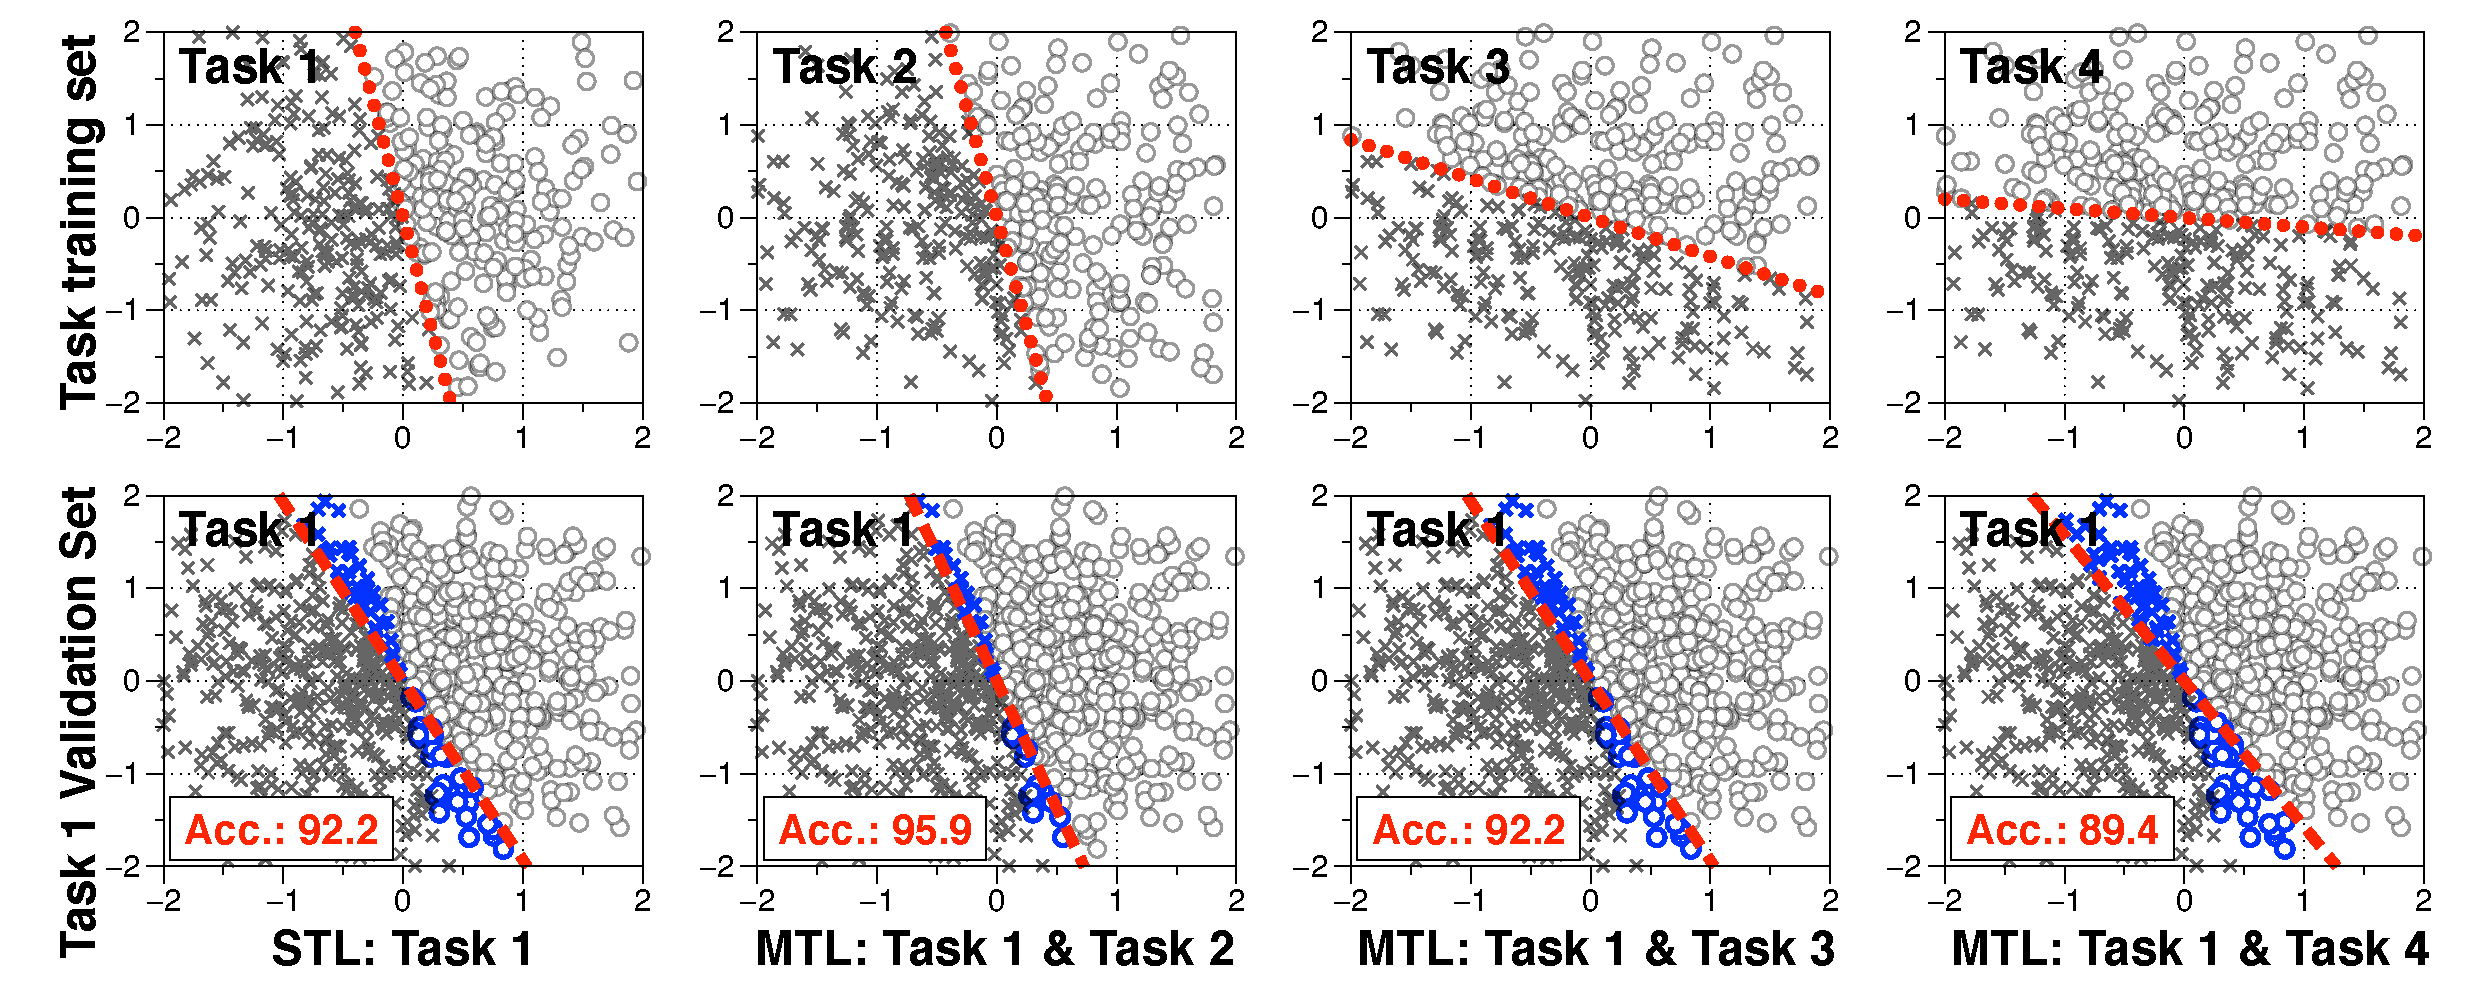
\includegraphics[width=0.8\textwidth]{figures/model_distance_motivation.pdf}
%	\caption{Positive to negative transfer as the source task rotates further away from the target task (left to right).}
%	\label{fig_motivation}
%\end{figure}


%We begin by observing that $\te(\hat{\beta}_t^{\MTL})$ can be decomposed into two parts, a variance part that is reduced from $\te(\hat{\beta}_t^{\STL})$, and a bias part that captures the difference between $\beta_t$ and the rest of $\beta$'s.
%	We term the bias part as .
%	Intuitively, whether $\te(\hat{\beta}_t^{\MTL})$ is lower than $\te(\hat{\beta}_t^{\STL})$ depends on the trade-off between the amount of variance reduced and the model shift bias part.
%	For the high-dimensional regime when $p$ goes to infinity, we derive the asymptotic limit of $\te(\hat{\beta}_t^{\MTL}) - \te(\hat{\beta}_t^{\STL})$ as a function of the number of datapoints $\set{n_1, n_2}$, the covariance matrices $\set{\Sigma_1, \Sigma_2}$, the ground truth parameters $\set{\beta_1, \beta_2}$, and a certain fixed value derived from solving equation \eqref{eq_mtl} (see Theorem \ref{thm_main_informal} for the statement).
%	While our focus is multi-task learning, our setup and technical tools are also applicable to transfer learning settings.
%	In Section \ref{sec_taskonomy}, we provide a case study of the
%	We observe a similar trade-off between model-shift bias and variance for this setting.
%	Based on the technical result, we provide theoretical insights over when multi-task learning performs better than single-task learning.


	We consider multi-task and transfer learning approaches to better understand when we should expect them to outperform single-task learning.
	We study the test performance of predicting a particular task given multiple tasks using a commonly used hard parameter sharing architecture.
	For the setting of linear regressions in the high-dimensional regime, we provide sharp bias-variance tradeoffs for multi-task and transfer learning estimators.
	A key technical tool that we develop is the trace of $(X_1^{\top}X_1 + X_2^{\top}X_2)^{-1}$ for two random matrices $X_1$ and $X_2$ in the setting of two tasks.
	Based on the theory, we provide more precise interpretations of many empirical phenomena in multi-task and transfer learning.
	For example, we quantify the benefit of multi-task learning for reducing the amount of labeled data, which is a key finding in Taskonomy by Zamir et al.'18.
	Finally, we show practical implications of our theory for detecting and improving negative effects in image and text classification tasks.





	We consider multi-task and transfer learning approaches to better understand when we should expect them to outperform single-task learning.
	We study the test performance of predicting a particular task given multiple tasks using a commonly used hard parameter sharing architecture.
	For the setting of linear regressions in the high-dimensional regime, we provide sharp bias-variance tradeoffs for multi-task and transfer learning estimators.
	A key technical tool that we develop is the trace of $(X_1^{\top}X_1 + X_2^{\top}X_2)^{-1}$ for two random matrices $X_1$ and $X_2$ in the setting of two tasks.
>>>>>>> 7e71ebba60efdaeeb1710c49d586517453dfabc2
	Based on the theory, we provide more precise interpretations of many empirical phenomena in multi-task and transfer learning.
	For example, we quantify the benefit of multi-task learning for reducing the amount of labeled data, which is a key finding in Taskonomy by Zamir et al.'18.
	Finally, we show practical implications of our theory for detecting and improving negative effects in image and text classification tasks.
%, i.e. %(following the argument of Proposition \ref{prop_monotone}), i.e.
%\[ \bigtr{(\hat{v}^2 X_1^{\top}X_1 + X_2^{\top}X_2)^{-1}\Sigma_2} \le \bigtr{(X_2^{\top}X_2)^{-1}\Sigma_2}. \]
%Because of model shift bias, we can no longer guarantee that $\te(\hat{\beta}_{t}^{\MTL}) \le \te(\hat{\beta}_t^{\STL})$.

%After describing this technical result, we provide theoretical insights over when multi-task learning performs better than single-task learning.
%Our analysis reveals three contributing causes of negative transfer, including task model \textit{dissimilarity}, \textit{unbalanced} data size, and \textit{covariate shift}, which we describe in detail for the rest of the section.


	%The test error $\te(\hat{\beta}_t^{\MTL})$, as a function of $M\in \cS_{\mu}$, is minimized at the identity matrix $\mu\id$ approximately by

%\be\label{formular_covariate0} (\te(\hat{\beta}_t^{\MTL}))(\mu \id) \le \left[1+ C\left(\frac{\rho_2}{\rho_1} + \frac{1}{\sqrt {\rho_1}}\right)\right]\cdot\min_{M\in \cal S_{\mu}}(\te(\hat{\beta}_t^{\MTL}))(M) ,\ee
%where the constant $C>0$ depends only on $\mu_{\max}$, $\mu_{\min}$ and $C_1$, but otherwise does not depend on $c_1$ and $c_2$.
	%is minimized when $M = \mu\id$.
